\documentclass[]{cwru}
\usepackage[acronym,shortcuts,nonumberlist]{glossaries}
\usepackage[toc,title]{appendix}
\usepackage{graphicx}
\usepackage{subcaption}
\usepackage[rightcaption]{sidecap} % Change if double-sided layout
\sidecaptionvpos{figure}{c}
\usepackage{color}
\usepackage{colortbl}
\usepackage{multirow}
\usepackage{longtable}
\usepackage{rotating}
\usepackage{array}
\usepackage{amsopn}
\usepackage{amssymb}
%\usepackage{hyperref}
\usepackage{amsthm}
\usepackage{amsmath}
\usepackage{mathrsfs}
%\usepackage{natbib}
\usepackage[square,sort,comma,numbers]{natbib}
\usepackage{complexity}
\usepackage{hyperref}
\usepackage[all]{hypcap}
\usepackage{epigraph}
\usepackage{algorithm}
\usepackage[noend]{algpseudocode}
%\usepackage{multipleinstance}
\usepackage{verbatim}
\usepackage{chronosys}
\DeclareMathOperator*{\argmin}{arg\,min}
\DeclareMathOperator{\atantwo}{atan2}
\MakeRobust{\Call}
\allowdisplaybreaks
\usepackage{tikz}
\usepackage{tkz-euclide}
\usetkzobj{all}
\usetikzlibrary{positioning,shapes.geometric,arrows,fit}
%\usetikzlibrary{bayesnet}
\tikzstyle{startstop} = [rectangle, rounded corners, minimum width=3cm, minimum height=1cm, text width=3cm, text badly centered, draw=black]
\tikzstyle{decision} = [diamond, aspect=2, minimum width=3cm, minimum height=1cm, text width=3cm, text badly centered, draw=black, inner sep=0pt]
\tikzstyle{sdecision} = [diamond, aspect=1.5, minimum width=3cm, minimum height=1cm, text width=3.5cm, text badly centered, draw=black, inner sep=0pt]
\tikzstyle{flowarrow} = [thick,->,>=stealth]
\tikzstyle{flowarrow} = [thick,->,>=stealth]

\tikzstyle{model} = [rectangle, rounded corners, minimum width=3cm, minimum height=1cm, text width=6cm, text badly centered, draw=black]
\tikzstyle{contribution} = [rectangle, minimum width=3cm, minimum height=1cm, text width=3cm, text badly centered, draw=black]

\definecolor{positivecolor}{RGB}{0,0,139}
\definecolor{negativecolor}{RGB}{139,0,0}
\definecolor{lightgray}{RGB}{215,215,215}

\def\checkmark{\tikz\fill[scale=0.4](0,.35) -- (.25,0) -- (1,.7) -- (.25,.15) -- cycle;}
\newcolumntype{C}[1]{>{\centering\let\newline\\\arraybackslash\hspace{0pt}}m{#1}}

\setlength\epigraphwidth{10cm}
\setlength\epigraphrule{0pt}

\setlength\LTcapwidth{\textwidth}

\definecolor{highlight}{rgb}{0.8,0.8,0.8}
\newcolumntype{g}{>{\columncolor{highlight}}c}
\newlength{\oldtabcolsep}
\newlength{\tabcaptionsep}
\setlength{\tabcaptionsep}{10pt}

\hypersetup{pdfborder=0 0 0,pdfview=FitH}
\fancyhead[LO,RE]{}% Remove section names from header

\renewcommand*{\acronymname}{List of Acronyms}
\renewcommand{\chapterautorefname}{Chapter}
\renewcommand{\sectionautorefname}{Section}
\renewcommand{\subsectionautorefname}{Section}
\newcommand{\Appendixautorefname}{Appendix}
% begin appendix autoref patch [\autoref subsections in appendix](http://tex.stackexchange.com/questions/149807/autoref-subsections-in-appendix)
\usepackage{etoolbox}
\makeatletter
\patchcmd{\hyper@makecurrent}{%
    \ifx\Hy@param\Hy@chapterstring
        \let\Hy@param\Hy@chapapp
    \fi
}{%
    \iftoggle{inappendix}{%true-branch
        % list the names of all sectioning counters here
        \@checkappendixparam{chapter}%
        \@checkappendixparam{section}%
        \@checkappendixparam{subsection}%
        \@checkappendixparam{subsubsection}%
        \@checkappendixparam{paragraph}%
        \@checkappendixparam{subparagraph}%
    }{}%
}{}{\errmessage{failed to patch}}

\newcommand*{\@checkappendixparam}[1]{%
    \def\@checkappendixparamtmp{#1}%
    \ifx\Hy@param\@checkappendixparamtmp
        \let\Hy@param\Hy@appendixstring
    \fi
}
\makeatletter

\newtoggle{inappendix}
\togglefalse{inappendix}
% end appendix autoref patch
\newcommand{\thesisstatement}[1]{\emph{#1}}
\newcommand{\mypar}[2]{\textbf{#1 (#2).}}
\DeclareMathOperator{\sign}{sign}
%% =================
%% Title Page Setup
%% =================

\makeatletter

\title{Interactive Feature Selection}
\author{Helen Zhao}
\date{}
\degree{Master of Science}
\doctype{dissertation}
\department{Electrical Engineering and Computer Science}
\defensedate{}

\begin{document}

\advisor{Dr.\ Soumya Ray}
\committee{}
\committee{}
\committee{}


\maketitle
\makeapprovalsheet

\frontmatter
\tableofcontents

\cleardoublepage
\phantomsection
\addcontentsline{toc}{chapter}{List of Tables}
\listoftables

\cleardoublepage
\phantomsection
\addcontentsline{toc}{chapter}{List of Figures}
\listoffigures

\begin{acknowledgments}

\end{acknowledgments}

\begin{abstract}

\end{abstract}

\mainmatter

\chapter{Introduction}
In machine learning, classification is the process of creating a model that maps the input data \(X=[x_1, x_2, ..., x_N]\) to output label \(y\). Classification algorithms are given training examples described by features \(X=[x_1, x_2, ..., x_N]\), which are measurements or observations of characteristics of the examples, and a target label \(y\), which is the variable to be predicted. The number of features can range from tens to hundreds depending on the problem domain. Not every feature provides information about the target, so instead a subset of informative features is used to create the model. Feature selection is the process of selecting the features to create the model and is an important step in the classification process. Feature selection improves prediction performance by removing irrelevant or noisy features, prevents overfitting to training examples, reduces computational cost of training, and identifies relevant features. Moreover, reducing number of features also reduces the amount of data collection and preparation because less training examples is required to create a generalizable model.\cite{ReviewOfFS,  IntroToFS}.

Feature selection directly effects the created model. Poor sets of features results in poor performing models. Selecting a set of informative features is a difficult problem. Exhaustive search of the feature subspace is costly and impractical. An exhaustive search for the optimal feature set of size \(k\), \(k < N\) would explore \(N\choose k\) possible feature sets. If the size of the feature set is also optimized, then there are \(2^N\) possible combinations of features. The number of combinations grows exponentially with dimensionality which makes the search for the optimal feature set NP-hard \cite{IntroToFS}.

While uncovering causal relationships between features is not required for finding predictive features, feature selection can benefit from the integration of causal discovery. Although conventional feature selection algorithms select features based on their effectiveness at predicting the target label, they may select features that are results of the experimental side effects rather than a property of the studied system \cite{CausalFS}. Furthermore, the user can build more understandable models that explain the underlying data generation mechanism by being aware of the cause and effect relationships in the data. 

\begin{figure}[h]
\centering
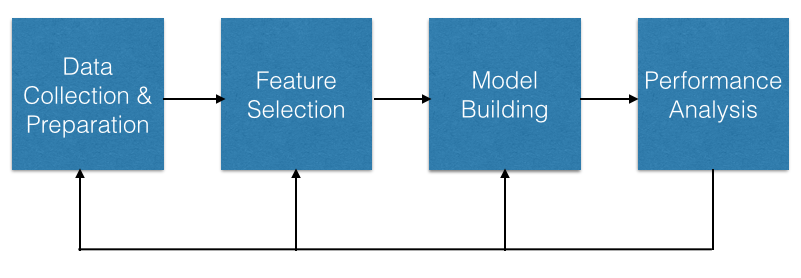
\includegraphics[width=1\textwidth]{MLflow}
\caption{ \textbf{Machine Learning Process.} Machine learning is typically an iterative approach. Many iterations are needed to create a model. The expert modifies inputs to the algorithm using the analysis of the current model's performance. From performance analysis, our system returns the user to feature selection step and allows the user to test a new feature set using newly acquired insights. }\label{fig:MLflow}
\end{figure}

We propose an interactive, iterative framework for feature selection that incorporates background knowledge. Machine learning is typically an iterative process consisting of data collection and preparation, feature selection, model creation, and performance analysis. In standard machine learning procedures, algorithms are often fully automated and domain expert’s contributions ends after collecting and preparing the data. Although the user can control the behavior of standard algorithms by tweaking input parameters, such as the depth of a decision tree, it is difficult to find the optimal parameter settings, which often change for different problem domains. As a result, the user has limited control and understanding of the algorithm. As opposed to automated machine learning, interactive machine learning engages user in generating the model. Furthermore, interactive machine learning is a natural method for integrating background knowledge. Interactions and interfaces can be designed to support efficient and effective communication between the expert and the algorithm. Moreover, an interactive approach can also account for the iterative aspect of model creation. 

We hypothesize that collaborative feature selection between the practitioner and learning algorithm will yield in a more understandable and higher performing model than non interactive feature selection techniques. Although computers are superior than humans at efficiently performing vast amounts of calculations, machine learning algorithms can still benefit from collaborating with humans. Domain experts have a rich understanding of the problem domain and the semantics of the input data, and interactive machine learning is a natural method for integrating prior knowledge that is difficult to express and encode in algorithms. Many of the classification datasets in the UCI repository have characteristics that can be explained to a human or understood by experts but are difficult to encode in a classification algorithm. 

To the computer, the characteristics are just rows and columns of numbers. The expert who often is involved in data collection and processing understands how the data values maps to real world situations and the meaning of the feature. An example is the meaning of the features in the breast cancer dataset built by Dr. Wolberg, a medical expert at the University of Wisconsin Hospitals. In the breast cancer data set, the feature clump thickness ranges from 1 to 10 and describes the extent to which the epithelial tissues lining the outer surface of the organ were one layered (1) or multilayers (10). Experts in breast cancer can map a value to its meaning in reality, understand the feature's relationship to other features and the possible implication a value has on the presence of breast cancer. Involving human in the feature selection process enables the user to interpret the model behavior and the predictions of individual examples.

Visual analytics is the use of interactive visual representations of data to gain insights into large, complex datasets. and can be used to help users efficiently gain insights into the data and the machine learning techniques. Visualizations is important tools for expressing information. Visual elements such as charts, maps, and graphs are often used to perform data analysis and gain insights about complex, high dimensional data that are difficult to manually analyze. Visualizations translate raw data into useful information that users are able to visually extract. For example, causal relationships is more easily communicated visually and are represented as directed acyclic graphs (DAG) where nodes represent features and direct edges represent cause and effect relationships as seen in figure \ref{CBN}. An integration of visual analytics techniques and classification methods can improve the the performance and transparency of the model created. Moreover, visual analytics can be used to facilitating communication and collaboration between the practitioner and the algorithm. Visualization can be used by both humans and machine to communicate information to each other in an efficient and effective manner. For example, users can interact with visuals to encode their soft knowledge in the visual system which can then translated the encoding to the algorithm. The algorithms uses the information provided by the user to perform calculations and can report the results to the user through visualizations.

In this thesis, we propose to perform feature selection as a collaborative effort between the user and the computer. For that purpose, we integrated feature selection techniques and visual analytics into a interactive visualization system. We devised a workflow that accumulates prior knowledge and incorporates the information into the exploration of possible feature sets. The user first encodes their background knowledge using interactive visualizations. The system expresses features visually, allows the user to interactively explore feature sets and build models from the feature set. Prior knowledge is incorporated in the exploration of feature space by calculating how consistent the feature subset is to the information previously provided by the user. Moreover, we incorporate performance analysis and design our system to account for the iterative nature of machine learning. The expert can create models and use their performance analysis to gain insights on other possible predictive feature sets; they can create many models and compare and contrast their performance and feature sets. We also present an evaluation of the effectiveness of the system in performing feature selection.

\indent Our contributions are a collaborative framework for feature selection that includes:
\begin{itemize}
  \item an interactive visualization for users to encode their prior knowledge about feature's relevancy to the target and a ranking of feature importance.
  \item a feature selection workflow that integrates causal discovery into the feature selection process and allows users to analyze causal networks and express their prior knowledge of causal interaction between features.
  \item an interactive visualization that enable users to dynamically explore possible feature sets and also communicates how consistent the feature set is to the prior information encoded.
  \item a performance analysis step that enable users to analyze the performance of models and compare the performance of models created from different feature sets.
\end{itemize}

Chapter 2 will provide necessary background knowledge on feature selection, visualization, and describe algorithms used in the thesis. It will also describe previously proposed and implemented visualization systems for machine learning. Chapter 3 describes the design and purpose of the interactive feature selection system. Chapter 4 describes the the design of the user study for evaluating the effectiveness and usefulness of the visual system. Chapter 5 presents the results of the evaluation study. Lastly, Chapter 6 presents conclusions, challenges and directions for future work.


\cleardoublepage
\chapter{Background and Related Work}
\indent This chapter introduces the context and background for this thesis.
\section{Interpretability}
\indent Machine learning practitioners have a wide palette of methods and tools. With advances in methodologies, practitioners are able to create high performing models for increasingly complex tasks and problems. A variety of models are produced from the diversity of machine learning algorithms and techniques. However, many models with impressively high performances are treated as black boxes - the information and reasons why they arrived at a prediction or decision is not transparent. An example of non-transparency is AlphaGo, a deep learner for playing the game Go, whose decisions for making moves in are unclear. \cite{InterpretDLModels}. The practicality of machine learning systems depends on whether humans can interpret and extract knowledge from the model and trust its predictions \cite{MakeMLInterpretable}. No matter how complexity or high performing the model is, if the system cannot explain its reasoning in a way the human can understand, humans can not act on the system’s decisions.

\indent In machine learning, a system is interpretable if is able to explain in understandable terms to humans. Researchers recognize the importance of interpretability and the amount of research in interpretable machine learning has grown along with surge in deployment of machine learning systems in all domains \citet{RigorousIntretable}. Doshi-Velez and Kim argue that interpretability is needed because problems are fundamentally under-specified. For example, an algorithm’s objective function may be slightly off from the target function and it is computationally or logically unfeasible to enumerate and test all possible inputs to a model. Therefore, the evaluation of an algorithm based on its optimization of the objective function is incomplete. Moreover, the ability to interpret the model is important for debugging, pinpointing the source of error and improve on the current model, and establish trust in the model. 
\section{Feature Selection}
\subsection{Problem Definition}
\indent Classification is the process of categorizing data points into a given set of categories. The category is also known as the target or the class label. The classification task is to approximate a mapping function from the input \(X=[x_1, x_2, ..., x_N]\) to the output class label \(y\) and creates a model that predicts the class label of a data point represented by a set of inputs also known as a feature vector. Features are measurable properties or characteristics that will help predict the target class. An example of a classification problem is predicting whether an email is spam or not spam. The target classes are spam and not spam, and features describing the emails can be word count, frequency of words, location email sent from, etc. 

\indent In supervised learning, we are provided with \(N\) features \(X=[x_1, x_2, ..., x_N]\), the target variable \(y\), and training examples drawn from the probability distribution of \(X\) and \(y\). Features are measurements or observations of properties and characteristics. The size of the feature vector varies from tens to hundreds or even more. The feature selection is the problem of selecting a subset of features in \(X\) to create a mapping to the target output \(y\) that will maximize the objective which is often the prediction performance of the constructed model on future examples.

\subsection{Introduction}
\indent Feature selection is performed before constructing a prediction model for many important reasons. Feature selection can help improve performance by removing irrelevant or noisy features and prevent overfitting to the training examples. Other benefits of feature selection include reduction in computational cost of training models and identification of features relevant or related to the target variable. Also less data is needed to be collected and processed because more training examples are required to create a generalizable model as the number of features increase. Moreover, a smaller feature set creates simpler models that are more easily interpreted by humans and explanatory of the underlying data generation mechanisms.  

\section{Common Feature Selection Strategies}
\indent An exhaustive search of an optimal feature set of size \(k\), \(k < N\) would explore \(N\choose k\) possible feature sets. If the size of the feature set is also optimized, then there is \(2^N\) possible combinations of features. The number of combinations grows exponentially with dimensionality making the search for the optimal feature set a NP-hard problem. Exhaustive search of the feature subspace is costly and impractical. Conventional feature selection strategies are composed of a search algorithm, an objective function to evaluate the feature subset, and a stopping criterion to stop the search. The search algorithm is independent of the evaluation function.

Two techniques for searching through the features subspace are feature ranking and subset search. In the feature ranking methods, features are ranked based on a merit value such as information content, entropy, relevance, etc. and the top \(k\) candidates are selected. The downside is that redundant and irrelevant features are not always removed. In subset search methods, the search process and elementary operations such as addition or removal of a feature to the current features subset are guided by the value of the objective function. The exploration can be computationally expensive with large feature sets and possible combination of features. 

The three main categories for feature selection approaches are filter, wrapper, and embedded. 
\subsection{Filters}
\indent Filters use the feature ranking technique to evaluate individual features or the feature subset based on measures of information, distance, consistency, similarity, and statistical measure \cite{ReviewOfFS}. Evaluation metrics are independent of the performance of the classifier. Filters can be easily used for most classifiers and useful for very high dimensional data because of their fast computation in comparison to the other two methods. However, the selected subset of features does not necessary build the best performing classifier because the evaluation metric may not relate to the performance of the classifier. A popular filter method is a Correlation based Feature Selection algorithm (CFS) proposed by Hall in 1996 \cite{FSAlgo} build on the heuristic that the features highly correlated with the target variable and uncorrelated with each other are good features for the problem. 

\subsection{Wrapper}
\indent Wrapper methods utilized the subset search technique. Since an exhaustive search for the optimal feature set is NP-hard, wrapper methods are suboptimal searches and some greedy method are on computational scale of \(O(N^2)\) \cite{Clopinet}. Forward selection start with an empty set and add features, while backward elimination start with a feature set and subsequently remove features. One example of wrapper method is forward feature selection, a greedy algorithm that starts with an empty feature set and iteratively adds the feature that would most improve an objective function. The classifier’s prediction performance is the common objective function guiding the search to the feature subset that would maximize the classifier’s performance. Wrapper methods can be used with most learning algorithm because the classifier is treated as a black box, but the resulting feature subset is optimal for the specific learning algorithm. A downside of wrapper methods is that the search space grows with the number of features and is computationally expensive because the classifier has to be reevaluated for every new subset of features and becomes unfeasible for large data sets and more computationally expensive learning algorithms. 
\subsection{Embedded and Hybrid}
Embedded methods incorporate or embed feature selection as a part of the learning algorithm. Various variants of decision tree algorithms, such as CART and random forest, are embedded methods. Hybrid methods combine the desired properties of filter and wrapper methods. A filter is first used to reduce the feature space and then a wrapper method is used to find the best feature subset.  

\section{Causal Feature Selection}
\indent Conventional feature selection algorithms in machine learning literature do not uncover causal relationships among features and between feature and target. Although discovering mechanisms not required for finding good predictors, awareness of cause and effect relationships can support in building more transparent model. Moreover by selecting features based on their effectiveness at predicting the target variable, feature selection algorithms may select feature that are the results of experimental side effects rather than a property of the studied system. The causal information provided by the selected features will help interpret the model’s predictions and make them more trustworthy. 

\indent Feature selection can benefit from causal discovery by revealing relevant features and increasing understanding of the data structure. The goal for the causal discovery problem is to discovery the causal relationship between features for a set of \(N\) input features \(X = [x_1, x_2, ..., x_n]\). The target variable is not singled out and any variable can be the target. 

\subsection{Causal Bayesian networks}
\indent Simple models of cause and effect relationship is based on Bayesian networks which aids in the understanding causality. Causal Bayesian networks is framework for representing the causal relationships for a set of random variables \(X = [x_1, x_2, ..., x_n]\) in the structure of a network. A Bayesian network is a directed acyclic graph (DAG) where each node map one to one to a variable in the set of variables \(X\). The Markov condition of Bayesian networks require every node to be conditionally independent of non descendent nodes given its parent node. A causal Bayesian networks is a Bayesian network where directed edges represent the relationship between variables. For all \(x_i\) and \(x_j\) in X, if there is a directed edge from \(x_i\) to \(x_j\), feature \(x_i\) is a direct cause of feature \(x_j\), then A directed path between two nodes indicates a causal relationship. Causal Bayesian network is a map of the dependencies and independencies of X. 

\subsection{d-separation}
Node \(x_i\) is d-separated from \(x_j\) by Z if Z is a set of node that blocks every path between \(x_i\) and \(x_j\). If \(x_i\) and \(x_j\) is not d-separated by C, then they are d-connected. In a causal Bayesian network, two nodes \(x_i\) and \(x_j\) is d-separated by Z if and only if \(x_i\) is conditionally independent of \(x_j\) given Z. \(x_i\) and \(x_j\) are d-connected \(iff\) they are conditionally dependent \cite{Clopinet}. 

\subsection{Markov blanket}
\indent The Markov blanket in a Bayesian network is the set of features that separates a given feature from the rest of the features in the graph. The Markov blanket is composed of direct causes (parents), direct effects (children), and direct causes of direct effects (spouses). Once all the direct causes of the target are known, indirect causes do not provide any additional information since their effect on the target is through a direct cause and captured in the direct cause. Although the children of the target are predictive of the target, knowing all the other causes of the target’s children (spouses) can help explain the amount of effect the target has on the children. The direct causes along with the direct effects of the direct causes enhance each others predictive power. Researchers has suggested that the Markov blanket for the target variable is an important concept for the feature selection problem \cite{MBforCL}. Feature relevant can be be described in relation to the Bayesian network. For any feature \(Y\), a irrelevant feature is disconnected from Y in the network. Features in the Markov blanket of \(Y\), \(MB(Y)\) are strongly relevant features. Features that are not in \(MB(Y)\) but have a directed path to Y are weakly relevant features \cite{Clopinet}. 

\subsection{Causal discovery algorithms}

\indent Learning causal relationships from observation data is a heavily researched area. The two parts of learning a Bayesian network are learning the structure of the graph G and the probability distribution of the variables. Algorithms for discovering the Markov Blanket that attempts to induce the complete causal Bayesian network does not scale with the increase in features. HITON is a more efficient method proposed for discovering Markov blanket \cite{HITON}. HITON first identifies the children and parents of the target. Then then identifies the children of the parent and the parent of the children of the target. Next, a wrapper method is used to search through the possible feature subset and return feature subset that resulted in the best performing classifier. 

\subsection{Greedy Equivalence Search}
The Bayesian network learning problem is to identify a DAG that fits the observed data \(D\) based on an objective function. The Greedy Equivalence Search (GES) algorithm \cite{GES} identifies an optimal structure and can be used to learn a causal network that fits the observed input data. For two DAGs \(H\) and \(G\), \(H\) is an independent map of \(G\) if the independence between variables implied by the structure of \(H\) is also implied by the structure of \(G\). For an independence map H of G, there exist a finite sequence of edge modification that can be applied to G such that after each edge modification H is still an independence map of G and at the end of the sequence G = H. H, G, and the intermediate DAGs G' are a part of the same equivalence class and are said to be equivalent. Meek proposed a two phase greedy algorithm that optimizes a Bayesian scoring function to find the network structure to map the observed data distribution. The algorithm starts with the equivalence class of DAGs that has no dependencies in the structure. In the first phase, edges are greedily added dependencies by considering all single edge addition that can be made to all the DAGs in the current equivalence class. After the algorithm stops at a local maximum, in the second phase, all single edge removals that can be made to all the DAGs in the current equivalence class are considered. The algorithm outputs the local maximum structure at the end of the second phase. Chickering \cite{GES} proved Meek's Conjecture and provided an implementation of GES. Later in the paper, we will be using a causal discovery tool \cite{Pycausal} implemented by the Center of Causal Discovery that performs GES.

\section{Visualization}
\subsection{Visual Analysis}
\indent Machine learning problems often use complex, multivariate data sets that are difficult to explore and gain insights from. When calculating aggregated statistical measures from large data sets, information is lost from oversimplification and misleading information is a common side effect. Visualization is one of the most relevant knowledge extraction method and can help translate raw data into useful information. Visualization of data helps communicates information and enhance people’s understanding of the data. Visual elements such as charts, graphs, maps can people visually and more efficiently identify trends, outliers, and patterns in the data. 

\indent Visual analytic is the combination of visualizations, human factors, and data analysis and the study of analyzing complex data set supported by interactive graphical and visual interfaces.
Although humans are significantly slower than computers, humans have soft knowledge that can not be expressed as inputs to an algorithm. While computers can performance fast calculations with numbers, the inputted data is all they know. For example, for machine learning classification models, the inputs are examples described by a set of features expressed in a table where rows are examples and columns are features. While the algorithm performs and optimizes calculations with the tabular data, the human has knowledge of the mapping from data values to situations in the real world and understand the rich information behind each feature. Furthermore, humans building the models often have a rich knowledge of the problem background and can catch spot mistakes the machines are making or the incorrect conclusions they may arrive at. Humans are also the ones judging whether the model is sensible in the end. Visual analytic is able to combine the computational and processing power of computers with the high visual processing power of humans and their prior knowledge of the problem. By allowing humans to interact with model, incorporate their prior knowledge, and analyze complex model through visual representations, they build a greater understanding of models and increase the trust of its predictions. 

\subsection{Visualization in Machine Learning}
\indent Visual analytic techniques and tools have been proposed and implemented for every step of the machine learning training process to support users in understanding, diagnosing, and improving models. Visualization systems have been created for specific machine learning models such as decision trees and neural networks and for specific domains such as natural language processing. For example, Stef van den Elzen created BaobabView \cite{BaobabView}, an interactive visual system for the construction and analysis of decision trees that incorporates the expert and their prior knowledge, and Yosinski released a software tool to study large deep learning networks through visualizing every neuron in a trained network as it responds to an input image \cite{Yosinski}. Another technique proposed to explain and visualize local explanations, the model’s output for a single example, to establish trust in a model’s predication. Tamagnini implemented Rivelo \cite{Tamagnini}, an explanation interface for interacting and exploring instance level explanation, which is the set of features that explains the prediction of an example. 

\subsection{Performance Analysis}
\indent Other visual systems extract knowledge from the model’s output to allow the users to interact with the visuals of the model’s output to evaluate its performance and explore and understand the model’s predictions. An example of performance analysis systems is ModelTracker \cite{ModelTracker} which lays out examples horizontally from low to high scoring examples to convey overall performance and enables users to directly interact and inspect examples for debugging. Also, Alsallakh created a system for visualizing probabilistic classification data that lays out histograms of prediction scores for each class in a circle to form a confusion wheel \cite{}. 
\indent I had proposed a set of visual methods that can facilitate analysis of the performance of probabilistic classifiers. The methods were integrated into Stacks, an interactive visual analytics system. Prediction scores are shown at the class level using histogram plots. Users can hone in on mistakes by filtering out irrelevant instances. The distribution of prediction scores communicates how confident the classifier is at its prediction. Furthermore, Stacks also incorporated error analysis for assessing why examples may be falsely classified or received a low prediction score.

\subsection{Visualizing for Feature Selection}
\indent Dimensionality reduction is a common strategy for reducing high dimensionality algorithm and to visualize and analyze high dimensional data in one, two, or three dimensional space. For example, t-Distributed Stochastic Neighbor Embedding (t-SNE) is a dimensionality reduction technique and useful for visualizing high dimensional data sets. 

Non-traditional methods of applying dimensional reduction has been implemented and utilizes visualization. Guo in 2003 \cite{Guo} implemented an interactive feature selection approach that uses visuals to identify patterns and feature subspaces from the high dimensional space. Every pair of features is represented in colored matrix where the color codes for the pair wise similarity. The matrix is sorted to highlight interesting clusters in feature subsets, and users can choose a reduced set of features to display the input data. Fernstad and Johansson created an interactive dimensionality reduction system \cite{InteractiveDR}whose process is influenced by the user. The user chooses the metric and parameters that the system uses to select the most import features and then the reduced features are displayed in a parallel coordinate visual or scatterplot matrix. Moreover, INFUSE \cite{INFUSE} is an interactive feature selection system that ranks features by its predictive power calculated across various feature selection algorithms and classifiers and visualizes the ranking in a sorted list. Users can select features to create their own model and compare their custom model to the other established feature sets.

\section{Evaluating Visual Systems}
\cleardoublepage
\end{document}

\backmatter
\cleardoublepage
\phantomsection-
\addcontentsline{toc}{chapter}{Bibliography}
\bibliographystyle{IEEEtran} 
\bibliography{thesis/thesis.bib}

\end{document}